\documentclass[a4paper,10pt]{scrartcl}
\usepackage[ngerman]{babel}
\usepackage[T1]{fontenc}
\usepackage[utf8]{inputenc}
\usepackage{graphicx}
\usepackage{float}

\title{Datenbanken 1}
\author{Benjamin Altmiks}
\date{10. Oktober 2018 - \today}
\begin{document}
\maketitle
\tableofcontents
\newpage
\section{Einleitung}
\subsection{Grundlagen und Basiskonzepte}
\subsubsection{Motivation}

\begin{itemize}
    \item Mehrbenutzerbetrieb
    \item Transaktionen (Deadlock Vermeidung) 
    \item Anweisungsorientiert (Eine Anweisung ganz oder gar nicht)
    \item Zugriffsrechte und Zugriffsmöglichkeiten
    \item Sicherungsmechanismus
\end{itemize}
\subsubsection{Datenbanken Terminologie}
\begin{enumerate}
    \item \textbf{Daten} sind Zeichen, die zum Zweck der Verarbeitung Informationen aufgrund bekannter oder unterstellter Abmachungen (Interpretationsregeln) darstellen.
    \item Ein \textbf{Datensatz} ist eine logische Zusammenfassung von Daten zu einer Einheit.
    \item Eine \textbf{Datenbank} (DB) ist ein integrierter, persistenter Datenbestand einschließlich aller relevanten Informationen(Metainformation)
    \item Ein \textbf{Systemkatalog}ist ein Verwaltungsinformationsrechner, der physische und logische Datenbankbearbeitung verwaltet. (Data Dictonary)
    \item Das \textbf{Datenbankverwaltungssystem(DBVS/DBMS)} ist die Gesamtheit aller Programme zum verwenden einer Datenbank
\end{enumerate}
Eine Datenbank besteht aus einem Datenbestand und seinem Systemkatalog und kann über ein DBMS im Datenbanksystem verwendet werden.
\begin{figure}[h]
	\centering
	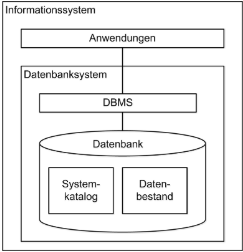
\includegraphics[width = 0.4\textwidth]{Grundaufbau.PNG}
	\label{img:grafik-dummy}
\end{figure}

\subsection{Architektur eines DBMS}
\subsubsection{3.Schema-Architektur (ANSI/SPARC)}
Besteht aus den drei Ebenen
\begin{itemize}
    \item Die externe Ebene = Struktur der Daten
    \item Die konzeptionelle Ebene = beschreibt den relevanten Informationsbereich
    \item Die interne Ebene = physische Abspeicherung und die Zugriffsorganisation
\end{itemize}

\subsubsection{Sprachschnittstellen}
\begin{itemize}
    \item \textbf{DML}(data manipulation language) = Eintrage, Ändern, Löschen mit Anfrage
    \item \textbf{DDL}(data definition language) = Umsetzung der Strukturen
    \item \textbf{DAL}(data administration language)= Speicherorganisation, Strukturumsetzung
\end{itemize}

\subsection{Datenmodell (DM)}
Ein formales Konzept der Beschreibung von Datenbankstrukturen
\begin{figure}[h]
	\centering
	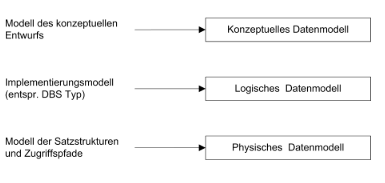
\includegraphics{Datenmodelle.PNG}
	\label{img:grafik-dummy}
\end{figure}

\subsubsection{Ebenen}
\textbf{Konzeptuelle Ebene}\newline
Beschreibungsmodell für Informationsstrukturen mit graphischer Notation
\newline\textbf{Logische Ebene}\newline Implementierungssicht, d.h Herleitung aus dem konzeptuellen Datenmodell 
\newline\textbf{Physische Ebene}\newline Verteilung der Daten auf Platen, also physische Speicherstrukturen
\subsubsection{Datenmodell-Typen} 
Satz- bzw. Tupelorientierte Beschreibungstechniken bei klassischen DM.\newline
Im Gegensatz dazu semantische DM mit Objekt- bzw. infromationsorientiert
\newline\textbf{Semantisches Datenmodell}\newline
Eine abstrakte, formale Beschreibung und Darstellung von Infromationen. Weitere Zerlegung der Darstellung nicht möglich (semantisch irreduzibel). Es zeigt die Beziehungen mithilfe von Modellierungskonstrukten dar.
\newline\textbf{Relationales Datenmodell} \newline
Ist die Darstellung von Datensätzen mithilfe von mathematischen Tabellen
\newline\textbf{Objektdatenmodell}\newline
Ein objektorientiertes Datenbankmodell verfolgt den Ansatz, Daten zusammen mit ihren Funktionen in einem Objekt zu speichern.
\newpage
\section{Modellierung}
Zum Übertragen von Daten ist es notwendig Information und Interpretationsregeln festzulegen. Erst dann kann eine Infromationsanalyse durchgeführt werden. Dafür müssen alle Sätze in semantisch irreduzible Sätze zerlegt werden. Ein Satz heißt semantisch irreduzibel, wenn er sich nicht ohne Informationsverlust in mehrere Sätze zerlegen lässt.
\subsection{Objekte und Analyse}
\subsubsection{Objekt- und Assoziationstyp}
Ein Objekttyp repräsentiert die Menge aller Objekte, die die gleiche klassifizierende Bedingung erfüllen. 
Objekttypen enthalten nur unterschiedliche Objekte. Das selbe gilt für Assoziationstypen (Beziehung).
\subsubsection{Rolle und Mitgliedschaft}
Die Rolle beschreibt den Beitrag eines Objekttypen zum Informationsgehalt eines Assoziationstypen. Ein Mitgliedschaftsintervall m:n (m: Untergrenze, n:Obergrenze) r bedeutet, dass ein Objekt des betreffenden Typs in mindestens m Assoziationen des Assoziationstyps auftreten muss bzw. in höchstens n Assoziationen auftreten darf.
\subsubsection{Lexikalisch}
Ein Objekttyp ist ein lexikalischer Objekttyp, wenn er durch einen Basistyp repräsentiert wird. 
Ein nicht-lexikalischer Objekttyp wird spezifiziert durch mindestens einen der nachfolgenden Punkte
\begin{itemize}
    \item Eine Namenskonvention
    \item Einen strukturierten Objekttyp
    \item Einen übergeordneten nicht-lexikalischen Objekttyp (Vererbung)
\end{itemize}
Lexikalische Objekttypen lassen sich durch Zeichen repräsentieren. 
Nicht-lexikalische Objekttypen nicht. Sie benötigen eine Namenskonvention.
\subsubsection{Namenskonventionen}
Die Namenskonvention legt fest, welche Assoziationen zur Identifikation eines Objektes dienen.
Der Assoziationstyp, der als Namenskonventionen festgelegt wird, hat die Mitgliedschaftsintervalle 1:1 und 1:1/0:1.
\subsection{System-/Basistypen}
Systemtypen stellen die Domänen des Systems dar. Alle möglichen Werte der Domänen sind Objekte des Systemtypen. 
Systemtypen sind Objekttypen. (String, Boolean)\newline  
Eine \textbf{Repräsentation} liegt vor, wenn ein Objekt durch ein Zeichen repräsentiert werden kann.  
\textbf{Basistypen} sind Objekttypen, die durch einen Systemtypen repräsentiert werden und alle Objekte aus dem Systemtypen übernehmen.
\subsection{Dreiecksbeziehung}
Ein Assoziationstyp ist eine benannte Beziehung zwischen n Objekttypen (n >= 2), die in dieser Beziehung bestimmte Rollen spielen.

\subsection{Vererbung}
Ein Objekttyp ist Untertyp eines anderen Objekttypen (Obertyp), wenn alle Objekte des Untertypen eine Teilmenge des Obertypen bilden. Man Unterscheidet zwischen verschiedenen Beziehungen zwischen Untertypen.
\begin{itemize}
    \item \textbf{or} = Die Untertypen können eine Schnittmenge haben
    \item \textbf{xor}= Die Untertypen sind gegenseitig exklusiv
    \item \textbf{and} = Die Untertypen haben dieselben Objekte
\end{itemize}
\subsection{Objektifizierung}
Ein Assoziationstyp kann gleichzeitig ein Objekttyp sein. 
Wird ein Assoziationstyp zum Objekttyp, so wird er objektifiziert. Dies wird objektifizierter Assoziationstyp bzw. strukturierter Objekttyp genannt.
\subsection{Konsistenzbedingungen}
Ein Assoziationstyp verknüpft mehrere Objekttypen. Die Konsistenzbedingungen zu einem Assoziationstyp spezifizieren die erlaubten Kombinationen von Objekten der beteiligten Objekttypen.\newline
\begin{figure}[h]
	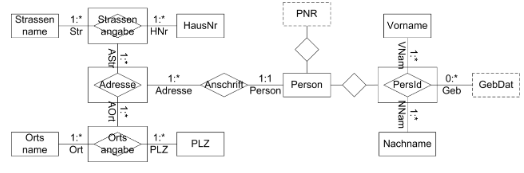
\includegraphics[width = 0.9\textwidth]{Informationsstruktur.PNG}
\end{figure}
\newpage
\section{Ableitung - Relationales Datenbankmodell}
\subsection{Logisches Schema}
Vorgehen:
\begin{enumerate}
    \item Zusammenhang durch 1:1 Verbindungen \\
    $\rightarrow$ Es werden alle engen Beziehungen markiert, also alle Verbindungslinien mit einem Mitgliedschaftsintervall 1:1
    \item Zusammenhang durch 0:1 Verbindungen \\
    $\rightarrow$ Allgemein definiert als enger Zusammenhang, also zu markieren. Es können in speziellen Fällen die Markierungen entfallen
    \item Zusammenhang durch Obertyp/ Untertypbeziehung \\
    $\rightarrow$ Obertyp-/Untertypbeziehungen stellen ebenfalls eine enge Beziehung zwischen den beteiligten Objekttypen dar. Würde eine Beziehung durch eine Assoziation dargestellt werden, so liegen Mitgliedschaftsintervalle von 0:1 bzw 1:1 vor, also eine enge Beziehung.
    \item Zusammenhangskomponenten \\
    $\rightarrow$ Verbundene/Markierte Objekt- und Assoziationstypen bilden gemeinsame Zusammenhangskomponenten. Es gibt dabei keine unmarkierte Verbindungen.
    \item Repräsentationen: Systemtypen und Basistypen \\
    $\rightarrow$ Repräsentationen benötigen keine Darstellung im logischen Datenmodell und werden bei der struktuellen Ableitung nicht berücksichtigt. 
    \item Objekttypen mit höheren Mitgliedschaftsintervallen\\
    $\rightarrow$ Streiche alle Objekttypen, die mindestens ein Mitgliedschaftsintervall mit der Untergrenze 1 haben! (Beziehung 0:x>1)
    \item Assoziationstypen \\
    $\rightarrow$ Zeichne eine Zusammenhangskomponente für alle Assoziationstypen, die keiner Zusammenhangskomponente angehören!
    \item Auflösung von Zyklen \\
    $\rightarrow$ Bei auftretenden Zyklen (markierte Verbindungen mit wiederkehrenden gleichen Rollen) müssen diese aufgelöst werden.
    \begin{itemize}
        \item (Falls vorhanden) 0:1 Markierungen werden gelöscht 
        \item UT-OT-Markierungen werden entfernt
        \item Wenn nur 1:1 Beziehungen, beliebig festzusetzende Markierung löschen
    \end{itemize}
    \item Verbindungen zwischen Zusammenhangskomponenten \\
    $\rightarrow$ Verbindungen zwischen Zusammenhangskomponenten zeigen auf, wie eine Zusammenhangskomponente in einer anderen referenziert wird. Diese sind zu markieren.
\end{enumerate}
$\rightarrow$ Im Ergebnis liegen alle Objekt- und Assoziationstypen entweder in einer Zusammenhangskomponente oder sie wurden gestrichen. Alle markierten Verbindungen liegen entweder in einer Zusammenhangskomponente (Markeirung des Zusammenhangs) oder sie verbindungen 2 Zusammenhangskomponenten (hier kann auch eine Zusammenhangskomponenten mit sich selber verbunden sein) (Markierung der Verbindung).
\subsection{Relationales Schema}
\begin{enumerate}
    \item Namen der Relationen \\
    $\rightarrow$ Markiere einen Objekttyp pro Zusammenhangskomponente (wenn nicht vorhanden: einen Assoziationstypen) als Name der Relation! Erstelle eine Liste der Relationen!
    
    \item Attribute für Objekttypen innerhalb der Zusammenhangskomponente \\
    $\rightarrow$ Füge zu den Relationen Attribute für innenliegende lexikalische Objekttypen hinzu und unterstreiche sie! (Objektifizierte Assoziationstypen sind lexikalisch) Untertypen zählen zu Objektobertyp, wenn keine eigene Repräsentation/Namenskonvention, ansonsten eigenes weiteres Attribut. 
    
    \item Attribute für Objekttypen außerhalb der Zusammenhangskomponente \\
    $\rightarrow$ Füge zu den Relationen Attribute für außenliegende Objekttypen mit Verbindung zu einem inneren Assoziationstyp hinzu. Unterstreiche das Attribut, falls das äußere Mitgliedschaftsintervall die Obergrenze 1 hat. Unterstreiche alle Attribute zusammen, wenn die Zusammenhangskomponente aus genau einem Assoziationstypen besteht.
    
    \item Ableitung von Obertyp-Untertyp-Konstrukten \\
    $\rightarrow$ Füge zu den Relationen, die getrennte Untertypen repräsentieren, eine vererbte Namenskonventionen hinzu!
    
    \item Zerlegung strukturierter Objekttypen \\
    $\rightarrow$ Zerlege strukturierte Objekttypen in die beteiligten Objekttypen! Führe dies fort, bis die abgeleiteten Attribute aus nicht strukturierten Objekttypen abgeleitet sind. Eigenschaften eines ersetzten Attributs werden für die Summe der ersetzenden Attribute übernommen.
    
    \item  Zerlegung strukturierter Objekttypen \\
    $\rightarrow$ Zerlege strukturierte Objekttypen in die beteiligten Objekttypen! Führe dies fort, bis die abgeleiteten Attribute aus nicht strukturierten Objekttypen abgeleitet sind. 
    
    \item Zusammenfassung von Attributen/Relationen \\
    $\rightarrow$ Fasse Relationen, die sich aus denselben Objektrollen ableiten, zusammen! Fasse gleichnamige Attribute in einer Relation zusammen!
    
    \item Schlüsselkandidaten\\
    $\rightarrow$ Ein Schlüsselkandidat liegt vor wenn:
    \begin{enumerate}
        \item Ein identifizierender innenliegender Objekttyp
        \item Bei strukturierenden Objekttypen alle hergeleiteten Attribute gemeinsam einen SK
        \item Für hergeleitete Attribute aus Objekttypen bilden alle Attribute gemeinsam ein SK
        \item Falls keiner dieser vorhanden, so bilden alle Attribute gemeinsam einen SK
    \end{enumerate} 
    
    \item Primärschlüssel \\
    $\rightarrow$ 
    Ein Primärschlüssel ist ein ausgewählter Schlüsselkandidat. Existieren in einer Relation mehrere Schlüsselkandidaten, so ist ein Schlüsselkandidat mit einem Mitgleidschaftsinterval 1:1 als Primärschlüssel auszuwählen. \\
    $\rightarrow$ 
    Kennzeichne alle Schlüsselkandidaten durch einfache Unterstreichung! Wähle die Primäschlüssel aus - kennzeichne sie durch doppelte Unterstreichung!
    
    \item Fremdschlüssel \\
    $\rightarrow$ Beziehungen zwischen Zusammenhangskomponenten sind durch Fremdschlüssel darzustellen. Dies können Objekt-Assoziationstyp Beziehungen wie auch Ober-Untertyp Beziehungen sein. Es gilt:
    \begin{enumerate}
        \item Objekt-Assoziationstyp: Assoziation referenziert Objekttypen. Attribut ist Fremdschlüssel auf Primärschlüssel oder beliebigen Schlüsselkandidaten.
        \item Obertyp-Untertyp: Untertyp referenziert Obertyp. Namenskonvention/Repräsentatoin ist der Fremdschlüssel auf Primärschlüssel oder beliebigen Schlüsselkandidaten.
        \item Sonderfall: Referenziertem Schlüsselkandidaten aus mehreren Attributen:
        $\rightarrow$ Fremdschlüssel in 2 Fremdschlüsselattribute aufteilen
    \end{enumerate}
    $\rightarrow$ Erzeuge für alle Beziehungen zwischen Zusammenhangskomponenten eine Fremdschlüsselbeziehungen!
\end{enumerate}
$\rightarrow$ Erzeuge für alle Beziehungen zwischen Zusammenhangskomponenten eine Fremdschlüsselbezihungen!
\newpage
\section{Relationale Datenbank}
\subsection{Transaktion}
Die Datenbank arbeitet anweisungsorientiert 
Eine Anweisung wird erfolgreich ausgeführt (ganz) oder sie wird mit einem Fehler beendet. Im Fehlerfall befinden sich die Daten im Zustand vor der Anweisung (gar nicht). \newline
$\rightarrow$ Eine Anweisung wird vom DBS ganz oder gar nicht ausgeführt.
TODO
\subsection{Transaktion ACID}
\begin{itemize}
    \item A - Atomicity (Atomizität) \newline
    $\rightarrow$ Alles oder nichts! Eine Transakton wird ganz oder garnicht bearbeitet
    \item C - Consistency (Konsistenz) \newline
    $\rightarrow$
    \item I - Isolation (Isolierung) \newline
    $\rightarrow$
    \item D - Durability (Dauerhaftigkeit) \newline
    $\rightarrow$
\end{itemize}
\subsection{Lock und Deadlock}
Zwischen den parallelen Transaktionen (verschiedener Benutzer) läuft eine pessimistische (vorbeugende) Synchronisation, die durch Sperren die Verzahnung der verschiedenen ändernden Zugriffe kontolliert, so dass die Transaktionsprinzipien garantiert werden können.
\newpage    
\section{SQL}
\subsection{DDL}
= Data Definition Language (Befehle zur Definition von Tabellen und anderer Datenstrukturen)
\subsection{DML}
Data Maniopulation Language (Befehle zur Datenmanipulation und Datenabfrage)
\subsubsection{SELECT}
\begin{verbatim}
    SELECT [FIRNR], [FIRUSER], [FIRTYP] FROM [dbo].[FIRMA];
\end{verbatim}
Diese Statement liefert alle Firmen, den jeweiligen Primärschlüssel, Firmenbezeichnung und Firmentyp, zurück
\subsubsection{INSERT}
\begin{verbatim}
INSERT INTO 
[dbo].[FIRMA]([FIRNR], [FIRUSER], [FIRTYP]) 
VALUES (1,'Musterfirma GmbH',0);
\end{verbatim}
\end{document}
